\documentclass[letterpaper,11pt]{article}
\usepackage[utf8]{inputenc}
\usepackage{amsmath, amssymb, graphicx, hyperref}
\usepackage{geometry}
\geometry{margin=1in}


\title{\vspace{-2.5em}\textbf{Volatility Models}}
\author{}
\date{\today}

\begin{document}

\maketitle
\vspace{-1em}
\hrule
\tableofcontents


\vfill
\section{Introduction}
For option pricing, volatility has always been an important parameter, especially since the introduction of the Black-Scholes model and the widespread use of implied volatility models. Whether analyzing past returns and market behavior or attempting to forecast future movements, mathematical models have played a crucial role in providing increasingly precise approaches.\\

Today, key models such as GARCH are used daily to price options at a fair value, balancing the interests of buyers and sellers. Which models are the most effective, and when should each of them be used ? What are their pros and cons, and which is better suited for specific purposes ?\\

In this document, we aim to provide a wider perspective on mathematical volatility models, exploring their features, applications, and limitations.

%\newpage


\section{Historical Volatility Models}

\subsection{Simple Moving Average (SMA)}
The Simple Moving Average (SMA) is one of the most basic methods for estimating historical volatility. It calculates the standard deviation of returns over a fixed number of past periods. For example, if we choose a 20-day SMA, we compute the standard deviation of the daily returns over the last 20 days. While this method is straightforward and easy to implement, it assumes equal importance for all observations in the selected window, which can sometimes make it less responsive to recent market changes.

\subsection{Exponentially Weighted Moving Average (EWMA)}
The Exponentially Weighted Moving Average (EWMA) model addresses the limitations of SMA by giving more weight to recent data points. This is achieved through an exponential decay factor, which ensures that older returns have progressively less influence on the volatility estimate. The smoothing parameter \( \lambda \), often set close to 0.94 in financial applications, controls how quickly the weights decay. EWMA is particularly useful for capturing shifts in market conditions as it adapts more quickly than SMA.



\subsection{Parkinson Volatility}
Parkinson volatility is a range-based measure that improves upon traditional volatility estimators by using the high and low prices of an asset over a specific period. Unlike methods that rely solely on closing prices, Parkinson's approach captures more information about price fluctuations throughout the trading day.

Parkinson volatility is given as:
\[
\sigma_P = \sqrt{\frac{1}{4n \ln(2)} \sum_{i=1}^n \left( \ln\left(\frac{H_i}{L_i}\right) \right)^2 }
\]

where:
\begin{itemize}
    \item \( H_i \) is the high price during the period,
    \item \( L_i \) is the low price during the period.
\end{itemize}

This estimator assumes no drift and that the price follows a Brownian motion. While Parkinson volatility is efficient for capturing intraday price movements, it may underestimate volatility if there are significant price jumps or if the closing price deviates substantially from the high-low range.



\subsection{Garman-Klass (GK) Volatility}
The Garman-Klass (GK) method is a range-based estimator of volatility that uses the high, low, opening, and closing prices of an asset within a specific period. This approach is more efficient than traditional methods because it incorporates more information from the price range rather than just closing prices. The GK estimator is defined as:
\[
\sigma_{GK}^2 = \frac{1}{n} \sum_{i=1}^n \left[ \frac{1}{2} \left( \ln\left(\frac{H_i}{L_i}\right) \right)^2 - \left(2\ln(2) - 1\right) \left( \ln\left(\frac{C_i}{O_i}\right) \right)^2 \right]
\]


where \( h \) and \( l \) are the natural logarithms of the high and low prices, and \( c \) is the natural logarithm of the closing price. By leveraging intraday data, the GK model provides a more accurate measure of historical volatility, particularly for assets with significant intraday price movements.





\subsection{Rogers-Satchell Volatility}
Rogers-Satchell volatility is another range-based estimator, but it accounts for potential drift in the price process, unlike Parkinson's method. This makes it more suitable for assets with trends, where the assumption of no drift may not hold.

The Rogers-Satchell volatility formula is:
\[
\sigma_{RS}^2 = \frac{1}{n} \sum_{i=1}^n \left[ \ln\left(\frac{H_t}{O_t}\right) \cdot \ln\left(\frac{H_t}{C_t}\right) + \ln\left(\frac{L_t}{O_t}\right) \cdot \ln\left(\frac{L_t}{C_t}\right) \right]
\]


where:
\begin{itemize}
    \item \( H_t \) is the high price on day \( t \),
    \item \( L_t \) is the low price on day \( t \),
    \item \( O_t \) is the opening price on day \( t \),
    \item \( C_t \) is the closing price on day \( t \).
\end{itemize}

This method is more robust than Parkinson volatility as it incorporates opening and closing prices, allowing for a more accurate representation of daily price movements and trends.



\subsection{Yang-Zhang Volatility}
The Yang-Zhang volatility model is a hybrid approach that combines the strengths of previous estimators, such as Parkinson and Rogers-Satchell, while addressing their limitations. It accounts for opening prices, closing prices, and intraday price ranges, making it one of the most accurate methods for estimating historical volatility.

The formula for Yang-Zhang volatility is:
\[
\sigma_{YZ}^2 = \sigma_o^2 + k \sigma_c^2 + (1 - k) \sigma_{rs}^2
\]

where:
\begin{itemize}

    \item $k = \frac{\alpha}{1 + n - \alpha}, \quad \alpha = 1 - \frac{2}{n}$

    \item \(\sigma_o^2\): The open-to-close variance: $\sigma_o^2 = \frac{1}{n-1} \sum_{i=1}^n \left( \ln\left(\frac{O_i}{C_{i-1}}\right) - \frac{1}{n} \sum_{i=1}^n \ln\left(\frac{O_i}{C_{i-1}}\right) \right)^2$
    
    \item \(\sigma_c^2\): The close-to-open variance: $\sigma_c^2 = \frac{1}{n-1} \sum_{i=1}^n \left( \ln\left(\frac{C_i}{O_i}\right) - \frac{1}{n} \sum_{i=1}^n \ln\left(\frac{C_i}{O_i}\right) \right)^2$

    \item \(\sigma_{rs}^2\): The Rogers-Satchell variance: $\sigma_{rs}^2 = \frac{1}{n} \sum_{i=1}^n \left[ \ln\left(\frac{H_i}{O_i}\right) \cdot \ln\left(\frac{H_i}{C_i}\right) + \ln\left(\frac{L_i}{O_i}\right) \cdot \ln\left(\frac{L_i}{C_i}\right) \right]$
    

    \item \(n\): Number of observations (e.g., days).
    \item \(O_i\): Opening price for the period.
    \item \(C_i\): Closing price for the period.
    \item \(C_{i-1}\): Closing price for the previous period.
    \item \(H_i\): High price for the period.
    \item \(L_i\): Low price for the period.
    
\end{itemize}


The Yang-Zhang model combines the open-to-close variance (\(\sigma_o^2\)), the close-to-open variance (\(\sigma_c^2\)), and the intra-day variance (Rogers-Satchell, \(\sigma_{rs}^2\)) to provide a robust estimate of volatility. This combination allows it to handle price gaps between consecutive days and intraday variations effectively.



\subsection{GARCH}
The Generalized Autoregressive Conditional Heteroskedasticity (GARCH) model is widely used for estimating and predicting volatility in financial time series. It builds on the idea that volatility is not constant but instead changes over time, often clustering during periods of market stress.

The GARCH model extends the simpler ARCH (Autoregressive Conditional Heteroskedasticity) model by including past conditional variances in the equation, making it more efficient for practical applications. The standard GARCH(p, q) model can be written as:

\[
\sigma_t^2 = \omega + \sum_{i=1}^q \alpha_i r_{t-i}^2 + \sum_{j=1}^p \beta_j \sigma_{t-j}^2,
\]

where:
\begin{itemize}
    \item \( \sigma_t^2 \) is the conditional variance (volatility squared) at time \( t \),
    \item \( r_{t-i}^2 \) are the squared past returns (shocks),
    \item \( \sigma_{t-j}^2 \) are the past conditional variances,
    \item \( \omega \) is a constant,
    \item \( \alpha_i \) and \( \beta_j \) are model coefficients, representing the weights of past shocks and variances, respectively.
\end{itemize}

The GARCH(1,1) model, the most commonly used variant, simplifies this to:

\[
\sigma_t^2 = \omega + \alpha_1 r_{t-1}^2 + \beta_1 \sigma_{t-1}^2.
\]

This model captures two key features of financial markets:
\begin{itemize}
    \item Volatility Clustering: Large changes in asset prices tend to be followed by large changes, and small changes by small changes, regardless of the direction.
    \item Mean Reversion: Volatility tends to revert to a long-term average over time.
\end{itemize}

GARCH is particularly valuable because it models conditional volatility, which adjusts dynamically based on new information, rather than assuming a constant level of risk. This makes it highly useful for risk management, option pricing, and forecasting future market behavior.

One limitation of the GARCH model is its symmetric response to positive and negative shocks, which fails to capture the "leverage effect" observed in financial markets. This has led to the development of extensions like EGARCH (Exponential GARCH) and TGARCH (Threshold GARCH), which incorporate asymmetry into the volatility estimation process.


\subsection{EGARCH}

The Exponential Generalized Autoregressive Conditional Heteroskedasticity (EGARCH) model is an extension of the traditional GARCH model. It is designed to address two key limitations of the standard GARCH framework: the inability to capture asymmetric volatility (the leverage effect) and the restriction of ensuring non-negativity of variances.

In the EGARCH model, the logarithm of the conditional variance is modeled as an autoregressive process. The formula for the EGARCH(1,1) model is given by:

\[
\ln(\sigma_t^2) = \omega + \alpha \frac{|z_{t-1}|}{\sqrt{\sigma_{t-1}^2}} + \gamma z_{t-1} + \beta \ln(\sigma_{t-1}^2),
\]

where:
\begin{itemize}
    \item \( \sigma_t^2 \) is the conditional variance at time \( t \),
    \item \( \omega \) is a constant term,
    \item \( \beta \) captures the persistence of volatility over time,
    \item \( \alpha \) measures the magnitude effect (how past shocks influence volatility),
    \item \( \gamma \) captures the leverage effect, which accounts for the asymmetry in volatility,
    \item \( z_t \) is the standardized residual, defined as \( z_t = \frac{\epsilon_t}{\sqrt{\sigma_t^2}} \), where \( \epsilon_t \) are the returns.
\end{itemize}

The use of the logarithmic form, \( \ln(\sigma_t^2) \), ensures that the conditional variance is always positive, eliminating the need for non-negativity constraints on the parameters.

Compared to standard GARCH models, EGARCH offers a more flexible and realistic framework for modeling financial time series data, especially in markets characterized by frequent and pronounced volatility shifts.



\newpage


\section{Implied Volatility Models}



\subsection{Black-Scholes}
The Black-Scholes model is one of the most famous tools in finance for pricing options. It assumes that the price of the underlying asset follows a geometric Brownian motion with constant volatility and no jumps. The formula for the price of a European call option under this model is given by:


\[
C(S, K, T, r, \sigma) = N(d_1) S_t - N(d_2) K e^{-rt} ,
\]

where:
\[
d_1 = \frac{\ln(\frac{S_t}{K}) + (r + \frac{\sigma^2}{2})t}{\sigma \sqrt{t}}, \quad d_2 = d_1 - \sigma \sqrt{t}.
\]



\begin{itemize}
    \item \( S_t \): Current price of the underlying asset.
    \item \( K \): Strike price of the option.
    \item \( t \): Time to expiration (in years).
    \item \( r \): Risk-free interest rate.
    \item \( \sigma \): Volatility of the underlying asset.
    \item \( N(\cdot) \): The cumulative distribution function of the standard normal distribution.
\end{itemize}

The model is powerful because it provides a closed-form solution for option prices, which can then be inverted to calculate implied volatility. However, its assumptions of constant volatility and log-normal price distributions often lead to inaccuracies in practice, particularly in markets with volatility smiles or skews.\\

\paragraph{BS PDE : }
\[
\frac{\partial V}{\partial t} + \frac{1}{2} \sigma^2 S^2 \frac{\partial^2 V}{\partial S^2} + r S \frac{\partial V}{\partial S} - r V = 0,
\]




\subsection{Stochastic volatility}

Stochastic volatility models are a type of models that assume both the asset price and its volatility are random processes. Unlike constant-volatility frameworks, these models introduce a separate stochastic process for volatility, often with mean-reverting behavior. Common formulations include models such as Stein-Stein, Hull-White, and others. These models help capture the dynamic nature of market risk and are widely used in pricing exotic options and managing risk, as they better reflect the empirically observed features such as volatility clustering and the leverage effect.\\



\subsection{SABR}
The SABR (Stochastic Alpha, Beta, Rho) model is widely used in the derivatives markets, especially for interest rate instruments, to capture the volatility smile. The model assumes that the forward price \(F_t\) and its volatility \(\sigma_t\) evolve according to the stochastic differential equations:
\[
dF_t = \sigma_t F_t^\beta\, dW_t, \quad
d\sigma_t = \nu \sigma_t\, dZ_t,
\]
with \(\mathrm{Corr}(dW_t,dZ_t)=\rho\), where:
\begin{itemize}
    \item \(\beta \in [0,1]\) controls the elasticity of the forward price,
    \item \(\nu\) is the volatility of volatility,
    \item \(\rho\) is the correlation between the asset and its volatility.
\end{itemize}



\subsection{Volatility Gamma}
Also known as the Variance Gamma (VG) model, this approach is a pure jump model that replaces the standard Brownian motion with a time-changed Brownian motion using a Gamma process. The log-return process in the VG model is given by:
\[
X_t = \theta G_t + \sigma W_{G_t},
\]
where:
\begin{itemize}
    \item \(G_t\) is a Gamma process with unit mean rate and variance rate \(\nu\),
    \item \(\theta\) represents the drift of the process,
    \item \(\sigma\) scales the Brownian motion \(W_{G_t}\) evaluated at the random time \(G_t\).
\end{itemize}
This framework captures skewness and excess kurtosis (fat tails) observed in asset returns, making it a powerful tool for option pricing and risk management when the assumption of normality isn't correct.


\subsection{Merton Jump Diffusion}
The Merton jump diffusion model extends the Black-Scholes framework by incorporating sudden, discrete jumps in the asset price along with the continuous diffusion process. The dynamics of the asset price \(S_t\) under this model are given by:
\[
\frac{dS_t}{S_t} = (\mu - \lambda \kappa)\, dt + \sigma\, dW_t + (J-1)\, dN_t,
\]
where:
\begin{itemize}
    \item \(\mu\) is the drift rate,
    \item \(\sigma\) is the volatility of the continuous part,
    \item \(W_t\) is a standard Brownian motion,
    \item \(N_t\) is a Poisson process with intensity \(\lambda\) representing the jump occurrences,
    \item \(J\) is a random variable representing the jump size, often assumed to be log-normally distributed,
    \item \(\kappa = E[J-1]\) is the expected percentage jump size.
\end{itemize}
By allowing for jumps, the model generates return distributions with heavier tails and higher kurtosis, which helps to explain market phenomena such as sudden price moves and volatility spikes.


\subsection{Heston Model}
The Heston model is a widely adopted stochastic volatility model that provides a semi-analytical solution for option pricing via characteristic functions. In the Heston framework, the asset price \(S_t\) and its variance \(v_t\) follow:
\[
dS_t = \mu S_t\, dt + \sqrt{v_t}\, S_t\, dW_t^S,
\]
\[
dv_t = \kappa (\theta - v_t)\, dt + \sigma \sqrt{v_t}\, dW_t^v,
\]
with \(\mathrm{Corr}(dW_t^S,dW_t^v)=\rho\), where:
\begin{itemize}
    \item \(\mu\) is the drift rate of the asset,
    \item \(v_t\) is the instantaneous variance,
    \item \(\kappa\) is the rate at which \(v_t\) reverts to its long-term mean \(\theta\),
    \item \(\sigma\) is the volatility of volatility,
    \item \(W_t^S\) and \(W_t^v\) are two correlated Brownian motions.
\end{itemize}
This model captures important market features such as mean reversion in volatility and the leverage effect.



\subsection{Surface Model}
Surface models focus on constructing the implied volatility surface, which represents the variation of implied volatility across different strikes and maturities. Rather than assuming a single volatility parameter, these models provide a comprehensive view of market expectations. Several approaches exist:
\begin{itemize}
    \item \textbf{Local Volatility Models:} Such as the Dupire model, which infers a local volatility function that is consistent with the observed market surface.
    \item \textbf{Stochastic Volatility Models:} Like the Heston or SABR models, which are calibrated to reproduce the surface dynamics.
    \item \textbf{Parametric Models:} For example, the Stochastic Volatility Inspired (SVI) parameterization offers a flexible yet parsimonious framework to fit the volatility surface.
\end{itemize}
\begin{center}
    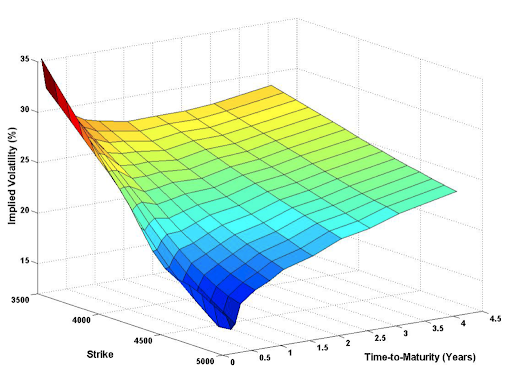
\includegraphics[width=0.8\textwidth]{img/vol_surface.png}
    \end{center}
These models are essential for pricing exotic options and performing robust risk management across different market conditions.

\subsection{Smile Model}
The volatility smile is an empirical pattern observed in options markets where implied volatility tends to be higher for deep in-the-money and out-of-the-money options than for at-the-money options. This deviation from the constant volatility assumption of the Black-Scholes model suggests that market participants expect a higher probability of extreme price movements. To capture this effect, several modeling approaches have been developed:
\begin{itemize}
    \item \textbf{Jump-Diffusion Models:} Such as the Merton jump diffusion model, which incorporate sudden jumps in asset prices.
    \item \textbf{Stochastic Volatility Models:} Like the Heston model, which allow volatility to change over time in a random manner.
    \item \textbf{SABR Model:} Provides an analytical approximation for the implied volatility smile, especially useful for interest rate derivatives.
\end{itemize}
By incorporating these dynamics, smile models help generate more accurate option prices and better reflect market risks.


\newpage

\section{Ressources}
\begin{itemize}
    \item \href{https://web-static.stern.nyu.edu/rengle/EnglePattonQF.pdf}{What good is a volatility model? - Robert F Engle and Andrew J Patton}
\end{itemize}

\bibliographystyle{plain}
\bibliography{volatility_models}


\end{document}
